% !TEX root = ../om_ts_04.tex

\begin{frame} % название фрагмента

\videotitle{Стационарные процессы}

\end{frame}



\begin{frame}{Стационарные процессы: план}
  \begin{itemize}[<+->]
    \item Определение стационарного процесса.
    \item Автоковариационная функция.
    \item Случайное блуждание и независимые величины. 
  \end{itemize}

\end{frame}

\begin{frame}
  \frametitle{Стационарный процесс}

  Случайный процесс с \alert{постоянными характеристиками}.
  \pause

  \begin{block}{Стационарность в широком смысле}
    Процесс $(y_t)$ стационарен в \alert{широком смысле}, если для любых $t$ и $k$:
    \[
    \begin{cases}
      \E(y_t ) = \mu \\
      \Cov(y_t, y_{t+k}) = \gamma_k \\          
    \end{cases}
    \]
  \end{block}

  \pause
  \begin{block}{Стационарность в узком смысле}
    Процесс $(y_t)$ стационарен в \alert{узком смысле}, если для любого $k$ 
    закон распределения вектора $(y_t, y_{t+1}, y_{t+2}, \ldots, y_{t+k})$ не зависит от $t$. 
  \end{block}
\end{frame}

\begin{frame}
  \frametitle{Стационарность: много уравнений}

  У стационарного процесса $(y_t)$:

  \[
  \E(y_5) = \E(y_7) = \E(y_{100}) = \E(y_{135}) = \ldots = \mu 
  \]
  \pause
  \[
  \Var(y_5) = \Var(y_7) = \Var(y_{100}) = \Var(y_{135}) = \ldots = \gamma_0 
  \]
  \pause
  \[
  \Cov(y_5, y_7) = \pause \Cov(y_8, y_{10}) = \pause \Cov(y_8, y_6) = \pause \ldots = \gamma_2 
  \]
  \pause
  \[
  \Cov(y_1, y_5) = \pause \Cov(y_8, y_{12}) = \pause \Cov(y_8, y_4) = \pause \ldots = \gamma_4 
  \]
  

\end{frame}


\begin{frame}
  \frametitle{Стационарный процесс: пример}

  \begin{block}{Независимые наблюдения}
    Величины $(y_t)$ независимы и одинаково распределены
    с конечным ожиданием $\mu_y$ и конечной дисперсией $\sigma^2_y$.
  \end{block}

  \pause
  \[
  \mu_y = \E(y_t)  
  \]
  \pause
  \[
  \gamma_0 = \Cov(y_t, y_t) = \Var(y_t) = \sigma^2_y.  
  \]
  \pause
  \[
  \gamma_k = \Cov(y_t, y_{t+k}) = 0, \text{ при } k \geq 1.  
  \]
\end{frame}


\begin{frame}
  \frametitle{Нестационарный процесс: пример}

  \begin{block}{Случайное блуждание}
    \[
    \begin{cases}
    y_0 = \mu \\
    y_t = y_{t-1} + u_t, \text{ при } t \geq 1 \\
    \end{cases},
    \]
    где $u_t$ — белый шум.
    \end{block}

  \pause 
  В явном виде: $y_t = \mu + u_1 + u_2 + \ldots + u_t$.    
  \pause
  \[
  \mu_y = \E(y_t)   
  \]
  \pause
  \[
  \gamma_0 = \Cov(y_t, y_t) = \Var(y_t) = \Var(\mu + u_1 + \ldots + u_t) = t\sigma^2_u.
  \]
  \pause
  \[
  \gamma_k = \Cov(y_t, y_{t+k}) = \Cov(y_t, y_t + u_{t+1} + \ldots + u_{t+k}) = \Var(y_t).
  \]
\end{frame}


\begin{frame}
  \frametitle{Случайное блуждание и случайная выборка}

  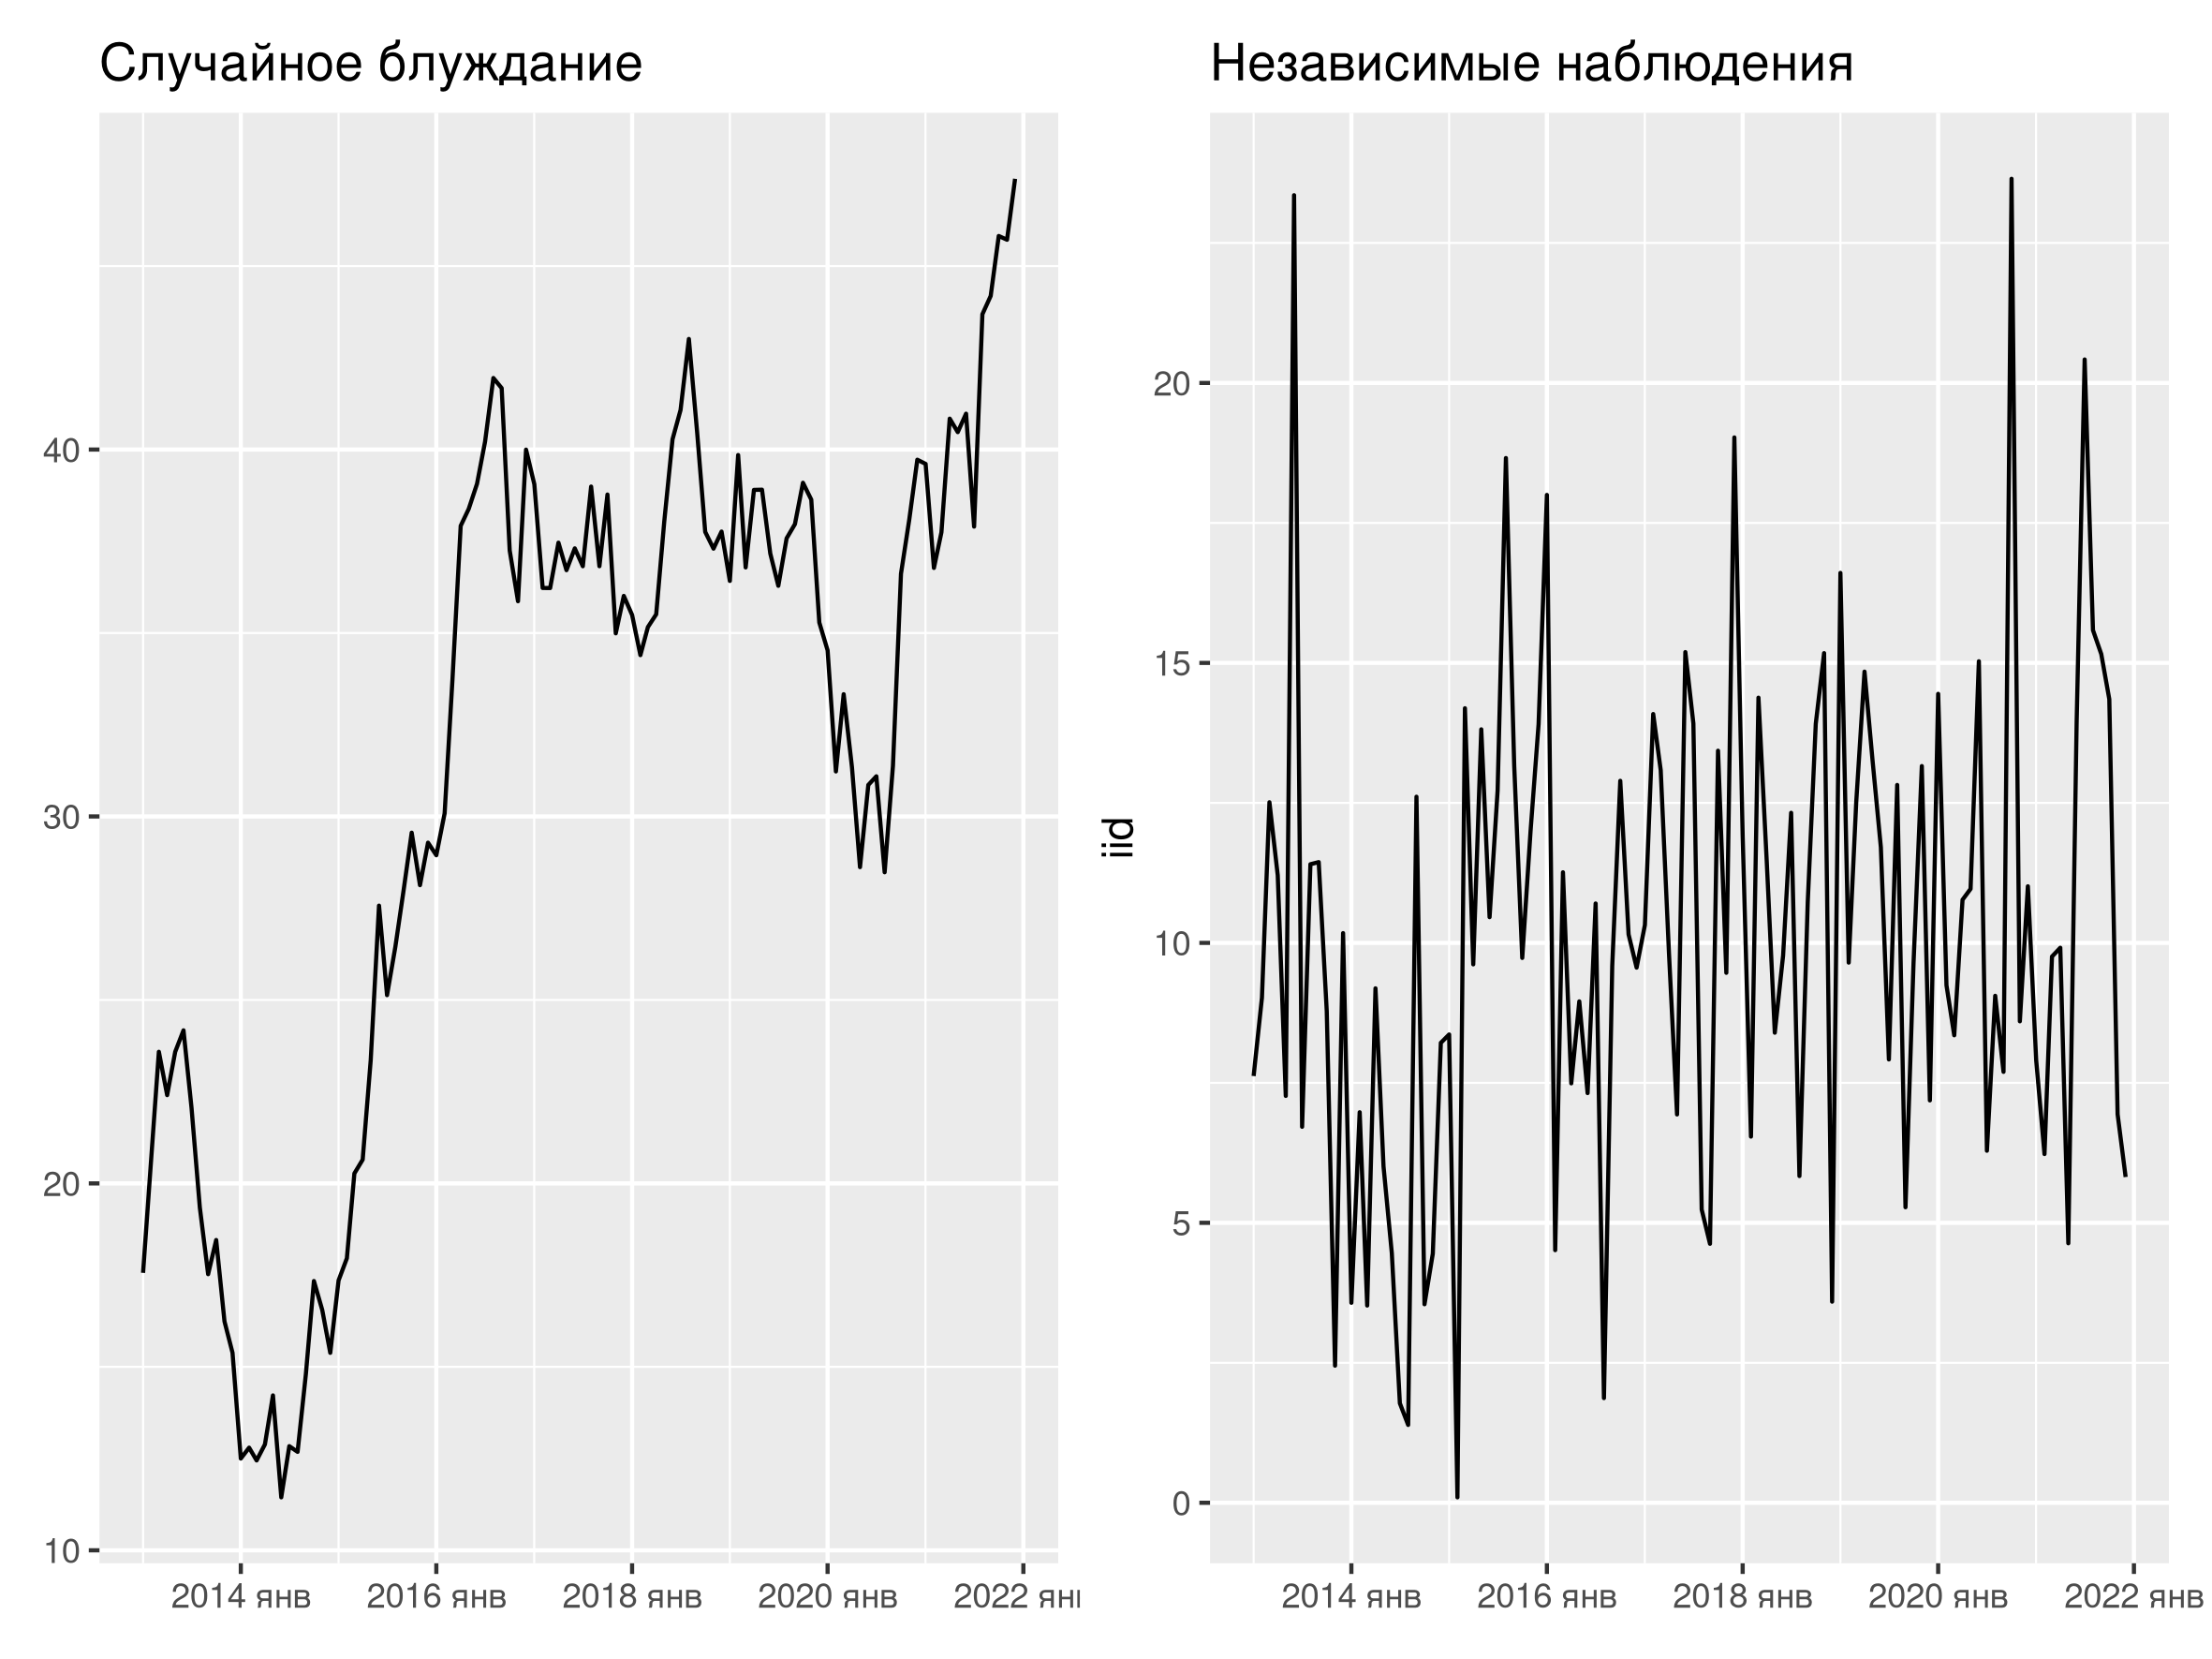
\includegraphics[width=\textwidth]{pictures/om_ts_04-028.png}


\end{frame}





\begin{frame}
  \frametitle{Автоковариационная функция}

  \begin{block}{Определение}
    Для стационарного процесса $(y_t)$ функцию $\gamma_k = \Cov(y_t, y_{t+k})$ 
    называют \alert{автоковариационной}. 
  \end{block}
  
  \pause
  \begin{block}{Определение}
    Для стационарного процесса $(y_t)$ функцию $\rho_k = \Corr(y_t, y_{t+k})$ 
    называют \alert{автокорреляционной}. 
  \end{block}
\end{frame}


\begin{frame}
  \frametitle{Связь функций}

\[
\rho_k = \Corr(y_t, y_{y+j}) = \frac{\Cov(y_t, y_{y+j})}{\sqrt{\Var(y_t)\Var(y_{t+k})}} =  \pause
\frac{\gamma_k}{\sqrt{\gamma_0 \gamma_0 }} = \frac{\gamma_k}{\gamma_0}
\]  

\end{frame}



\begin{frame}
  \frametitle{Автоковариационная функция — наше всё!}

  \begin{block}{Теоремка}
    Если вектор $(y_t, y_{t+1}, \ldots, y_{t+k})$ имеет многомерное нормальное распределение 
    при любом количестве компонент, то константа $\mu = \E(y_t)$ и функция $\gamma_k = \Cov(y_t, y_{t+k})$
    полностью определяют конечномерные распределения случайного процесса $(y_t)$.
  \end{block}

\end{frame}



\begin{frame}{Стационарность: итоги}

  \begin{itemize}[<+->]
    \item Постоянные $\E(y_t)$, $\gamma_k = \Cov(y_t, y_{t+k})$.
    \item \alert{Автоковариационная} функция. 
    \item Случайное блуждание нестационарно. 
    \item Случайная выборка стационарна.
  \end{itemize}
\end{frame}

